\newpage
\section{coquillage}

\begin{figure}[h]
    \centering
    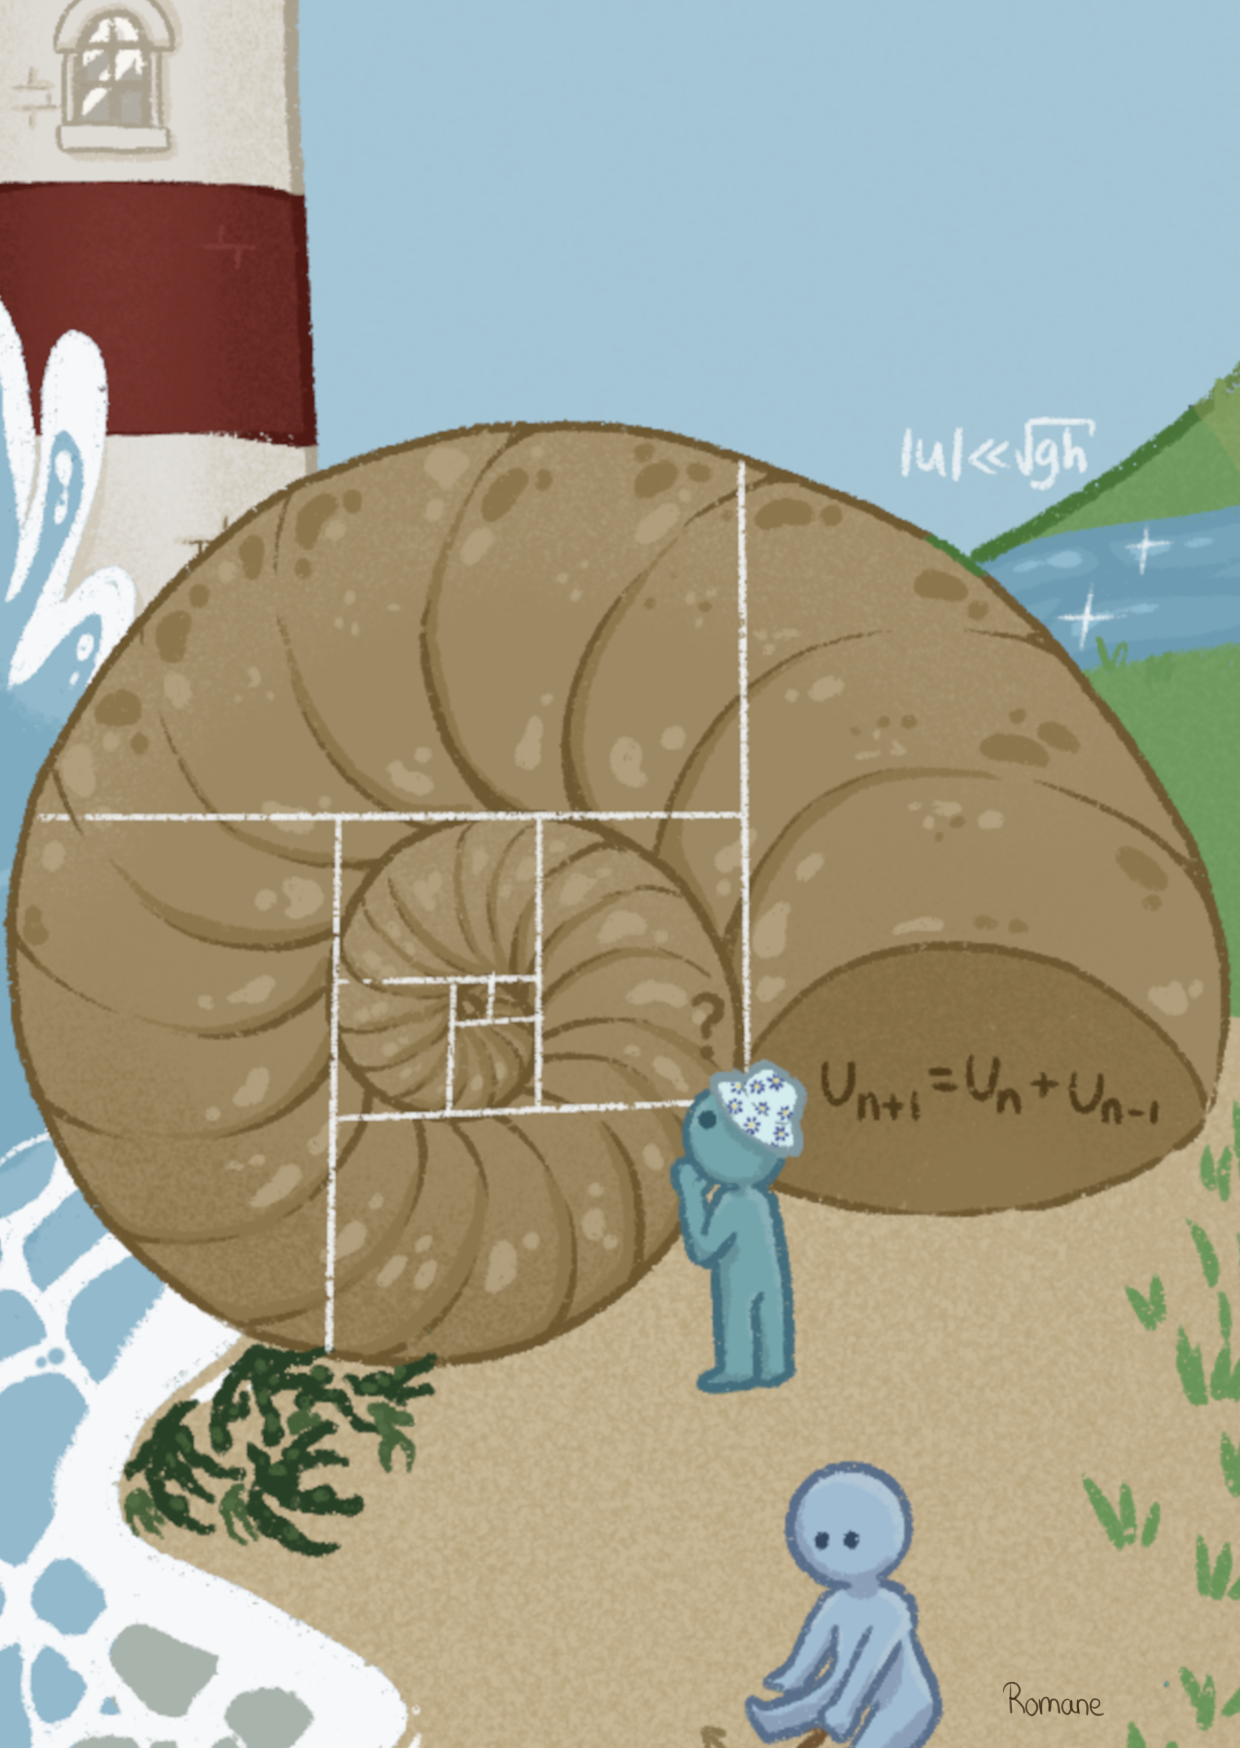
\includegraphics[height=0.5\textheight]{Cartes_postales/carte02-coquillage.png}\label{fig:c02}
    \caption{Carte postale: Coquillage}
\end{figure}

Les mathématiques nous aident à décrire les formes du vivant. Par exemple, le coquillage de la nautile a une forme de spirale logarithmique. La nautile crée sa coquille au fil de sa croissance, en l'élargissant et l'enroulant sur elle-même. Cette forme mathématique peut s'agrandir autant qu'on veuille en gardant exactement la même forme (plus précisément, cela revient à la tourner d'un certain angle). Si on zoom ou dézoom sur la spirale, on voit exactement la même chose, juste tourné un peu.

\medskip

Cette propriété est cruciale car elle permet aux nautilles de grandir sans devoir changer de forme ou créer une nouvelle maison tous les 3 mois. De plus, cette spirale est equiangle, la courbe s'éloigne du centre de manière très régulière, ce qui la rend très résistante à la pression. La pression se répartit uniformément sur tout le coquillage car il n'y a aucune partie plus fragile qui risque de céder en premier. Ceci lui permet de plonger très profondément mais aussi de resister à des prédateurs.

